%%%%%%%%%%%%
%
% $Autor: Wings $
% $Datum: 2019-03-05 08:03:15Z $
% $Pfad: Functions.tex $
% $Version: 4250 $
% !TeX spellcheck = en_GB/de_DE
% !TeX encoding = utf8
% !TeX root = manual 
% !TeX TXS-program:bibliography = txs:///biber
%
%%%%%%%%%%%%

\chapter{Assembly}

\section{Assembly}

The mobile robot is assembled following the SparkFun JetBot AI Kit v2.0 hardware guide, which describes how to mount the NVIDIA Jetson Nano A02, camera, battery, and accessories on the two-plate chassis \cite{SparkFunJetBotAssembly:2020}.
The lower plate holds the \acs{dc} motors, wheels, and basic chassis structure, while the upper plate carries the NVIDIA Jetson Nano A02 Developer Kit and Qwiic expansion hardware \cite{SparkFunJetBotAssembly:2020}.
Assembly uses standard M3 hardware and a small Phillips screwdriver, and no soldering is required because all electrical interconnects are provided through Qwiic cables and ribbon connectors \cite{SparkFunJetBotAssembly:2020}.

The camera assembly step mounts the Leopard Imaging IMX219 Camera module onto the front camera bracket using the supplied screws and standoffs \cite{SparkFunJetBotAssembly:2020}.
The bracket is then fixed to the front edge of the top plate so that the camera optical axis points forward and slightly downward toward the floor \cite{SparkFunJetBotAssembly:2020}.

\begin{figure}[H]
	\centering
	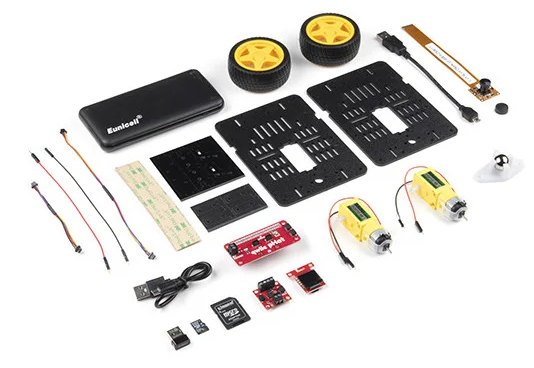
\includegraphics[width=0.72\textwidth]{Images/Hardware/jetbotpartslayout}
	\caption{Main mechanical and electronic parts of the SparkFun JetBot AI Kit before assembly.\cite{SparkFunJetBotAssembly:2020}}
	\label{fig:jetbot-parts-layout}
\end{figure}



\begin{figure}[H]
	\centering
	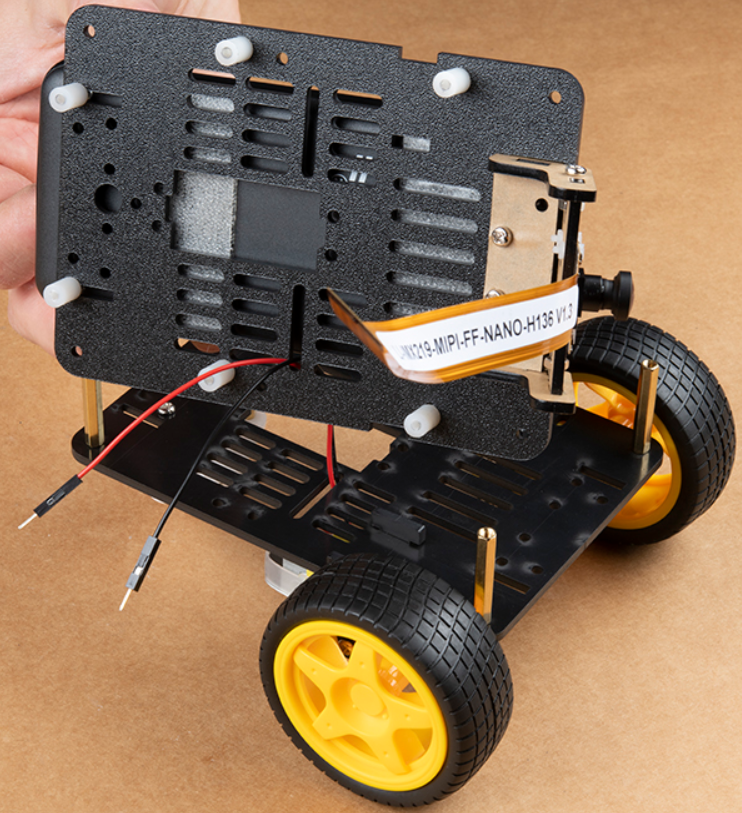
\includegraphics[width=0.72\textwidth]{Images/Hardware/jetbotaccessories.png}
	\caption{Top-plate accessory installation showing Leopard Imaging IMX 219 Camera and cable routing.\cite{SparkFunJetBotAssembly:2020}}
	\label{fig:jetbot-top-accessories}
\end{figure}


\begin{figure}[H]
	\centering
	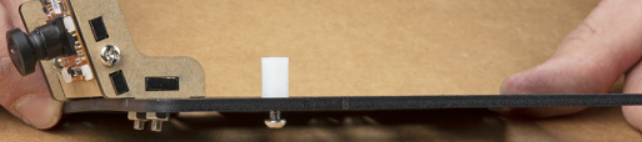
\includegraphics[width=0.62\textwidth]{Images/Hardware/jetbotcameramount.png}
	\caption{Front camera bracket and \acs{csi} ribbon installation on the JetBot chassis.\cite{SparkFunJetBotAssembly:2020}}
	\label{fig:jetbot-camera-mount}
\end{figure}

The CSI ribbon cable is routed from the camera to the NVIDIA Jetson Nano A02 camera connector, taking care to avoid sharp bends and to maintain the correct connector orientation \cite{NVIDIA:2019}.
Cable slack is managed so that the ribbon does not obstruct the field of view or interfere with wheel motion \cite{SparkFunJetBotAssembly:2020}.



\begin{figure}[H]
	\centering
	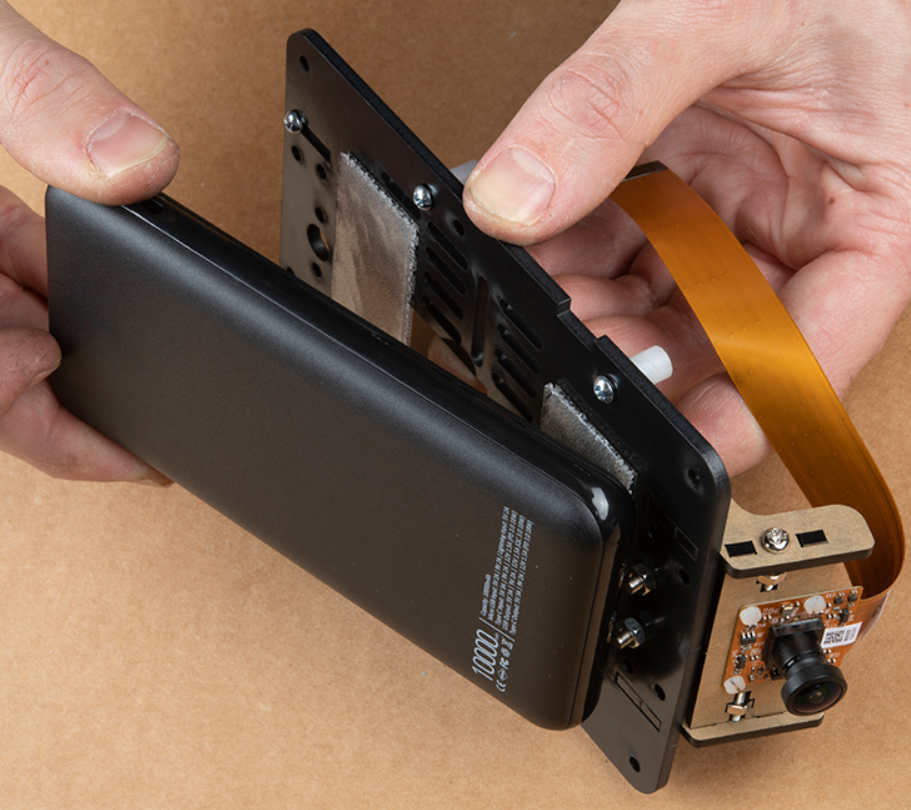
\includegraphics[width=0.72\textwidth]{Images/Hardware/jetbotbatterymount.png}
	\caption{Mounting Battery \cite{SparkFunJetBotAssembly:2020}}
	\label{fig:mount-battery}
\end{figure}


The Eunicell \acs{usb} power bank is mounted on the top plate in the updated assembly configuration rather than underneath the chassis \cite{SparkFunJetBotAssembly:2020}.
This placement improves access to the power button and charge port and avoids reducing ground clearance.\cite{SparkFunJetBotAssembly:2020}
Velcro straps or elastic bands secure the battery pack to the top plate so that it cannot slide during acceleration or collision tests. \cite{SparkFunJetBotAssembly:2020}.
The \acs{usb} cable from the battery pack is plugged into the Jetson Nano power input as specified in the assembly guide to provide sufficient current during peak load \cite{SparkFunJetBotAssembly:2020}.

Accessory installation continues with mounting the SparkFun Qwiic Motor Driver and SparkFun Micro \acs{oled} Breakout on the top plate around the NVIDIA Jetson Nano A02 \cite{SparkFunJetBotAssembly:2020}.
The Qwiic pHAT is connected to the 40-pin header on the NVIDIA Jetson Nano A02 and secured using the included standoffs so that Qwiic connectors remain accessible \cite{SparkFun:2019a}.
Short Qwiic cables connect the pHAT to the motor driver and the Micro OLED, forming the local I\textsuperscript{2}C interconnect on the upper deck \cite{SparkFunJetBotAssembly:2020}.
The motor driver output terminals are wired to the left and right \acs{dc} motors, and polarity is selected so that positive commands correspond to forward motion on both sides \cite{SparkFun:2019b}.

Once all components are mounted, the top plate is attached to the lower chassis using the supplied standoffs, producing a rigid two-level robot structure \cite{SparkFunJetBotAssembly:2020}.
Final checks include verifying that all screws are tightened, wheels rotate freely, connectors are seated properly, and the camera view remains unobstructed \cite{Siegwart:2011}.


\begin{figure}[H]
	\centering
	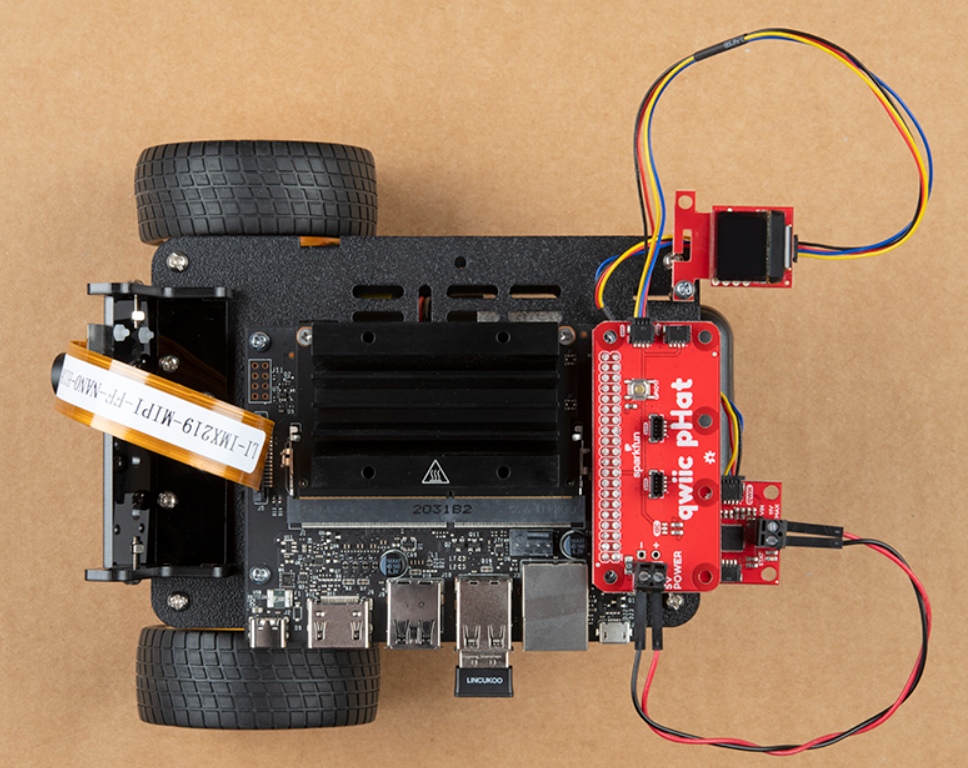
\includegraphics[width=0.66\textwidth]{Images/Hardware/jetbotfinalassembly.png}
	\caption{Fully assembled SparkFun JetBot \acs{ai} Kit used as the mobile robot platform \cite{SparkFunJetBotAssembly:2020}.}
	\label{fig:jetbot-final-assembly}
\end{figure}

Only after the mechanical assembly passes these checks is the system powered on for software setup and calibration \cite{SparkFunJetBotAssembly:2020}.



\section{Assembly Best Practices}

\begin{itemize}
	\item Ensure camera lens is clean and properly focused before assembly
	\item Mount camera on a stable platform to minimize vibration during motion
	\item Verify motor encoder alignments for accurate odometry
	\item Use vibration-damping materials between compute platform and chassis
	\item Keep cable routing organized to avoid mechanical interference
	\item Test all connections before final enclosure
\end{itemize}

\section{Component Verification}

\begin{itemize}
	\item Motor responses should be immediate and smooth
	\item Camera stream should display without artifacts or lag
	\item Encoder pulses must be consistent during calibration runs
	\item Power delivery should be stable under full load
\end{itemize}


\section{Component Functions in Localization Context}

\subsection{Camera Module}
\begin{itemize}
    \item Captures 30 fps video stream for feature extraction
    \item Provides environmental context for visual odometry
    \item Enables loop closure detection through image similarity
\end{itemize}

\subsection{Motor and Encoder System}
\begin{itemize}
    \item Propels robot along desired trajectory
    \item Encoders count wheel rotations for incremental odometry
    \item Enables dead reckoning between visual updates
\end{itemize}

\subsection{Jetson Nano Compute Platform}
\begin{itemize}
    \item Processes images at real-time frame rate
    \item Solves pose graph optimization problems
    \item Maintains feature descriptor database for loop closure
\end{itemize}

\section{Sensor Synchronization}
All sensors must be synchronized to timestamp events correctly. Motor encoders provide synchronous pulses; camera frames are timestamped on capture. 
\subsection{Next Steps}
Follow Domain Hardware and Domain Software in Thesis Report for more guided Software installation, testing and calibration of the Mobile robot.

